\chapter{CRM AI: An use case} \label{chapter:use-case}

One of the goals of this project is to integrate an artificial intelligence solution within a CRM. After the analysis of \textit{CRM AI}, it has been decided to develop a predictive machine learning model based on CRM data. This part has been developed in collaboration with one of ELCA's client, hereafter referenced as \textit{Company A} \footnote{Client name and business subject to confidentiality.}.

This chapter \ref{chapter:use-case} details this machine learning project. Sections \ref{sec:use-case} and \ref{sec:ml-metrics} explains the problem \textit{Company A} is currently facing and how a machine learning solution might solve it.The data to feed the machine learning comed from Company A's CRM, as explained in section \ref{sec:crm-data}. Section \ref{sec:ml-experimentation} details the machine learning experimentation and models used. Once the model has been trained and tested, it was integrate within Company A's CRM, as outlined in section \ref{sec:crm-deployment}. Finally, sections \ref{sec:use-case-further-work} and \ref{sec:use-case-conclusion} conclude this part with a reflection on the entire initiative.

% -------------------------------- Section: Client's use case
\section{Client's use case} \label{sec:use-case}
\textit{Company A} is a global energy enterprise active overall Switzerland. It offers several products and services and one of those is subject to a very tense market, where the characteristics of the product are the same for all companies and the price is the only difference between competitors. Therefore, several specificity of this product must be taken into account:
\begin{itemize}
\item This product is classified as a safety need in Maslow's hierarchy of needs\cite{wiki:Maslow's_hierarchy_of_needs}, meaning that people don't buy it because the \textit{like} it but rather because they \textit{need} it. 
\item Due to its classification in Marslow's hierarchy, the product is usually stored in high quantities. Typical customer will make a large order, fill their supplies and once fully consumed, buy back the product, again in large quantities. Therefore, the product is not buy on a daily basis, more on an annual-basis. This complicates the job of Company A to build customer loyalty.
\item As product's characteristics are the same for all, the price is the only variable that companies can \textit{play} with. Nevertheless, a part of the price is subject to market variation, from which companies will adapt their margins. As all stock market, the prices can vary, even marginally, each day.
\end{itemize}

 Based on these particularities of the product, building a solid customer relationship is difficult for \textit{Company A}. Customers only need to make one order per year and their are usually not subject to an immediate need. Therefore, they can take the time to compare the price offered by all suppliers in the market and place an order accordingly. This facts explain why \textit{Company A} is often dealing with \textit{one-time customers} and experiences a high customer turnover \textbf{[ADD DATA SUPPORING THAT CLAIM]}.
 
 
 To counter this customer churn, \textit{Company A} is building \textit{customer recovery} plans to get back lost clients as well as interactions with other products and services to build an ecosystem of offers, but they want something uniquely targeting their key-product. Currently, Company A marketing team are contacting clients with annual newsletters. Those newsletters are send to each client every year around the same period. The company wants to strengthen this marketing process by contacting clients at the perfect time, before they start to search for offers from the competition. This will enable Company A to retain clients and ultimately build customer loyalty.
 
 
% -------------------------------- Section: Project outline
\section{Formalize machine learning problem} \label{sec:ml-metrics}

As defined in section \ref{sec:use-case}, the goal of this initiative is to build a machine learning model that predicts the time of a customer's next order. This problem can be formalize as a regression problem, for which the machine learning model will output the date of next order: at date $d$, the model will predict $i$, the number of days until next order. So $d+i$ will give the precise data of customer next order. Variants are to define $i$ as the number of weeks or months until next order. The date will be less precise but the predictions might turn out to be more satisfying. Another possibility is to formalize it as a classification task and output a binary value to the question : \textit{"Will this customer make an order in the coming day/week/month ?"}. After discussion with \textit{Company A}, it has been decided to define the output of the model as \textit{the number of months until customer next order}. In details, it has been decided first to work with regression models to have multiple ranges of outputs. Then, for the output's granularity (day, week or month), predicting the number of month until next order \textit{should} give stronger results. It will allow \textit{Company A} to asses how well a regression techniques are suited for this problem and, in a second phase, trying to have more precise predictions, with an output at the week level for example.

From the machine learning output, Company A wants to reach customers before they make an order. The process is planned as follow:
\begin{enumerate}
    \item At the beginning of each month, compute the predictions for all active clients\footnote{An client is flagged as inactive if no more business can be made with him/her (moving abroad or death for example)}.
    \item Retrieve all clients with a predictions smaller than $2$.
    \item Get in touch with these clients if and only if they have not been contacted in the past two months.
\end{enumerate}
The last step of this process is very important, as it will ensure that the company won't reach the same client twice.


Now that the machine learning goal and usage have been specified, the metrics for its success must be defined. As stated above, this is a regression model, where the output will be a real number. Usual metrics for regression problems like Mean Absolute Error (MAE) or Root Mean Squared Error (RMSE) are not well suited for this project and for the usage of the predictions by \textit{Company A}. As specified above, the company plans to get in touch with a client only if the predictions is below $2$. Therefore, if the output of a model is equal to $7.0$ months or $4.35$, it ends up being the same for \textit{Company A}. This explains why RMSE or MAE cannot be used to evaluate machine learning models performance. As regression metrics are not applicable, the models will be assess with custom metrics inspired by classification problems: precision, recall and F1 score. 

To transform the regression problem into a classification one, model's predictions will be classify into one of the following four classes: \texttt{0, 1, 2 or 3+}. The class \texttt{0} is meant for predictions between 0 and 1 (excluded) - clients that should make an order in the current month. Same idea for classes \texttt{1} and \texttt{2}. The class \texttt{3+} regroups all predictions with an output bigger or equal to 3 - client next order should occur in three or more months.

\begin{adjustwidth}{-1cm}{}
    \begin{minipage}[b]{0.60\linewidth}
    \resizebox{1.0\columnwidth}{!}{
        \begin{tabular}[t]{c|c|
                >{\columncolor[HTML]{EFEFEF}}c|c|
                >{\columncolor[HTML]{EFEFEF}}c }
                Customer & y\_true & y\_true class & y\_pred & y\_pred class \\ \hline
                A        & 2       & 2             & 3.32    & 3             \\
                B        & 0       & 0             & 0.4     & 0             \\
                C        & 0       & 0             & 0.1     & 0             \\
                D        & 5       & 3+            & 2.9     & 2            \\
                E        & 3       & 3+            & 0.8     & 0             \\
                F        & 1       & 1             & 1.6     & 1             \\
                G        & 1       & 1             & 0.8     & 0             \\
                H        & 2       & 2             & 1.4     & 1             \\
                I        & 9       & 3+            & 15.2    & 3+            \\
                J        & 0       & 0             & 2.5     & 2            
        \end{tabular}
        }
        \captionof{table}{Example of output truth and predictions}
        \label{table:example_truth_preds} 
    \end{minipage}
    \hspace{1.0cm}
    \begin{minipage}[b]{0.45\linewidth}
        \offinterlineskip
        \moveright 1cm \hbox{\raisebox{1.8cm}[10pt][10pt]{\rotatebox[origin=c]{90}{\parbox[c][0pt][c]{15cm}{True class\\[50pt]}}}\par}
        \hspace*{1cm}\MyHBoxT[\dimexpr5.1cm]{Predicted class}\vspace*{-0.4cm}
        \hspace*{1cm}\MyHBox{0}\MyHBox{1}\MyHBox{2}\MyHBox{3+}\vspace*{-0.2cm}
        \MyTBox{0}{2}{0}{1}{0}
        \MyTBox{1}{1}{1}{0}{0}
        \MyTBox{2}{0}{1}{0}{1}
        \MyTBox{3+}{1}{0}{1}{1}
        \captionof{table}{Confusion matrix for table \ref{table:example_truth_preds}}
        \label{table:example_confusion_matrix} 
    \end{minipage}
\end{adjustwidth}


Based on this classes assignment, a confusion matrix can be generated. Then, custom metrics inspired by precision, recall and F1-score are computed:
\begin{itemize}
    \item \textbf{Precision}: Of all clients that make an order in the current month, how many where predicted with class 0 or 1? This metric computes the percentage of true orders catch by the model. 
    $$ Precision = \frac{t_0\_p_0 + t_0\_p_1}{t_0\_p_0 + t_0\_p_1 + t_0\_p_2 + t_0\_p_{3+}} $$
    
    For the example in table \ref{table:example_confusion_matrix}, the precision is equal to $\frac{2+0}{2+0+1+0} = 0.667$
    
    \item \textbf{Recall}: From all clients that the model has predicted an order for the current month, how many did actually made an order in the current or coming month? The goal with this metric is to assert that the model is not always predicting 0, which will give a precision score of 100\%, but will make \textit{Company A} contact all clients. 
    $$ Recall = \frac{t_0\_p_0 + t_1\_p_0}{t_0\_p_0 + t_1\_p_0 + t_2\_p_0 + t_{3+}\_p_0} $$
    
    For the example in table \ref{table:example_confusion_matrix}, the recall is equal to $\frac{2+1}{2+1+0+1} = 0.75$
    
    \item \textbf{F1-score}: Same as the F1-score for classification tasks. 
    $$ \fscore = \frac{2*Precision*Recall}{Precision+Recall} $$

    For the example in table \ref{table:example_confusion_matrix} the F1-score is equal to $\frac{2*0.667*0.75}{0.667+0.75} = 0.71$
\end{itemize}

In the formulas above, $t_i\_p_j$ correspond to the sum of true orders occurring in \texttt{i} months and predicted to occur in \texttt{j} months. For example $t_0\_p_0$ corresponds to the count of orders occurring in the current month and predicted as such (top left case in the confusion matrix).

The metric \textbf{F1-score} will be the benchmark metric for this project.

% -------------------------------- Section: Data
\section{Data from CRM} \label{sec:crm-data}

This section outlines the data gathering, cleaning, transformation and feature engineering processes. Before doing some machine learning experiments, a first goal is to understand the data and figure out the main factors that push a client to make an order. For the analysis of data and machine learning experiments, the development has been done within \textit{Jupyter Notebooks} with a \texttt{Python 3} kernel, mainly relying on the \textit{Pandas} package.

Data comes from \textit{Company A} CRM, a Dynamics 365 Online instance. By using to the \textit{Web Api} offered by Dynamics 365, all entities of the CRM have been retrieved and analyzed. From the 291 entities present in the CRM, only a few are useful for this project: \texttt{Orders}, \texttt{Accounts}, \texttt{Contacts} and \texttt{Buildings}. The relationships between those entities are straightforward: An order must be linked to an account and each account is linked to at least one contact, one of which must be the \textit{primary contact}. The \texttt{Contact} entity models a real person, where the \texttt{Account} entity models a customer of \textit{Company A}, either a person or a company. Contacts can then be linked to one or more instance of the \texttt{Building} entity.

\begin{figure}[h]
    \centering
    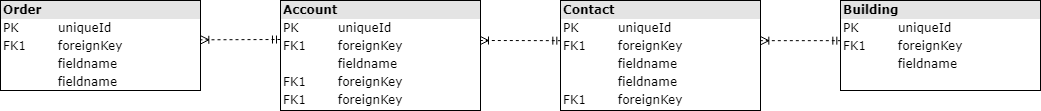
\includegraphics[width=15cm]{images/entityDiagram.png}
    \caption{Entity Diagram for \textit{Company A} CRM data - \textbf{TODO}}
    \label{fig:entity-diagram}
\end{figure}

\subsection{Orders}\label{sec:crm-orders}

The \texttt{Order} entity holds all information about an order made by an account. The CRM contains all orders received by \textit{Company A} since 2013 until nowadays. For this project, all orders considered ranged from January 2013 until June 2018, included. Once the raw data has been downloaded from all \texttt{Orders} entities, the first steps are to clean this set of 808'532 orders. Indeed, even if a CRM save its data in an organized manner and Dynamics 365 has some verification upon data entry, mistakes can still happen when a person enters data into the system. Orders have been discarded based on their names -empty or not-, on their status -active or not- and on their internal characteristics (amount delivered equal to zero, delivery date in 1956, delivery date occurring before the order date, ..). This cleaning phase removes 28.79\% of the orders, which gives a data set of 575'679 orders, each order having 37 features.

All these orders have been made by 183'706 accounts, with a mean of 3.14 orders per account and a median of 2. Grouping accounts per the number of orders made reveals that 50.77\% of accounts is this dataset have made one or two orders\footnote{Accounts which have made at least one order since 2013 - Figure \ref{fig-annex:orders_per_accounts} in the annexes.}. This demonstrates the singularity of a very competitive market in which clients often change their suppliers and fully benefit from the competition. In respect to the machine learning model, it will be very difficult to extract some common behavior and generalize, due to the low amount of orders for those accounts. Therefore, accounts with less than three orders have been discarded, leading to a dataset composed of 451'986 orders (-21.49\%).

As traditional accounts only order once per year, there is a seasonality effect visible when plotting the number of orders per month trough the years (figure \ref{fig:order_per_monthyear}). Even if the periodicity of orders isn't regular, a year experiences two pics of orders: one around March and another around October. On the opposite side, there have been fewer orders in Spring, around the month of June. The data plot in figure \ref{fig:order_per_monthyear} indicates that the weather must play a crucial order when accounts are making orders - it's colder in March and October than in June. As detailed in further section \ref{sec:external-data}, the model will take some weather-related information into consideration.

\begin{figure}[h]
    \centering
    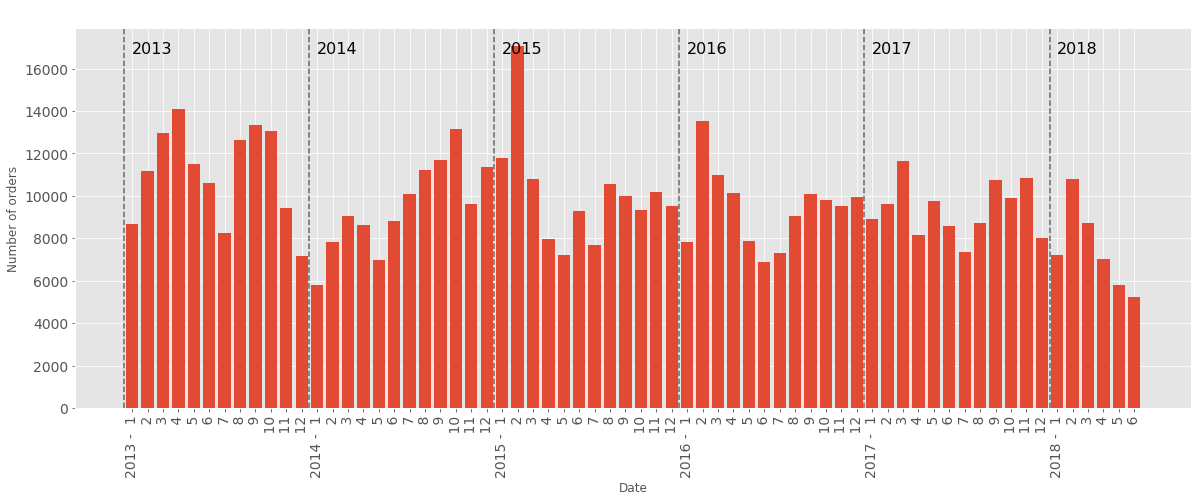
\includegraphics[width=15cm]{images/order_month_year.png}
    \caption{Number of orders per month per year}
    \label{fig:order_per_monthyear}
\end{figure}


As stated above, a typical customer will make an order once per year, with a number of months between two orders around 12 months, as presented in figure \ref{fig:orders-account-counts}. A mean of 12.67 months and a median of 11 months are retrieved by computing the average "wait" time between two orders for all accounts. Figure \ref{fig:orders-account-counts} shows that there is a lot of accounts waiting 11 months between two orders, but there is also account which order more frequently. On the other side, the number of accounts waiting 13 or more months between two orders decreases. Within this plot, there are two pics: the first one logically around 11 months and a second one around 23 months. This second pic is probably due to "jumper accounts", accounts that order one year with \textit{Company A}, the following year with the competition and, two years after they first orders, order again with \textit{Company A}. 

\begin{figure}[h]
    \centering
    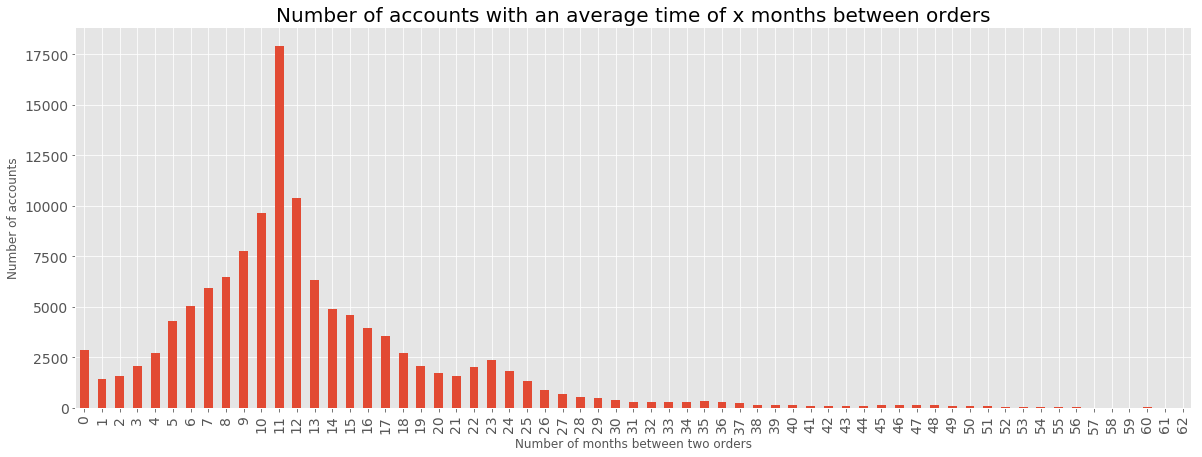
\includegraphics[width=15cm]{images/accounts-average-time-orders.png}
    \caption{Accounts grouped by the average number of months between two orders}
    \label{fig:orders-account-counts}
\end{figure}

This plot also reveals \textit{key-accounts}, accounts ordering at least once per month. Those accounts are most of the time companies, considered as very regular customers by \textit{Company A}. As detailed in section \ref{sec:data-shape-for-ml}, \textit{key-accounts} will not be a problem for the machine learning model.


\subsection{Accounts, Clients and Buildings}\label{sec:crm-accounts}
The \texttt{Account} entity holds information related to the clients of \textit{Company A}, either a natural or legal person. Due to imports from a legacy system, the Dynamics 365 instance of \textit{Company A} contains more than 1'100'000 accounts. Filtering those accounts based on the final orders from section \ref{sec:crm-orders} gives 88'552 accounts, with 244 features per account. The company stocks a lot of account properties in their CRM and the vast majority of those are null or not useful for this next order prediction task. After a review of all these features, only 11 will be kept, among which account's activeness and account's name, which will be compared to it's primary client name.

Indeed, all accounts are linked to a primary contact. The \texttt{Contact} entity holds information about a physical person, like its address or phone number. From this entity, only two features will be used: the birth date and the name. The birth date will be used to see if the age of a person as an influence on it's buying habits. The contact name will be use in comparison with the account name. As mentioned above, the \texttt{Account} entity can be a natural or a legal person, but there is no feature in the CRM to specify this account state. As this information is important -a legal person can make orders on a very frequent basis- such feature is built. An account's name can be compared to the name of its primary contact. If both names are equal, the account will be considered as a natural person, otherwise the account will be considered as a legal person, assuming that an account modelling a legal person will not have the same name as it's primary contact. As shown in figure \ref{fig:account-contact-name-orders}, accounts classified as a legal person made orders much more frequently.

\begin{figure}[h]
    \centering
    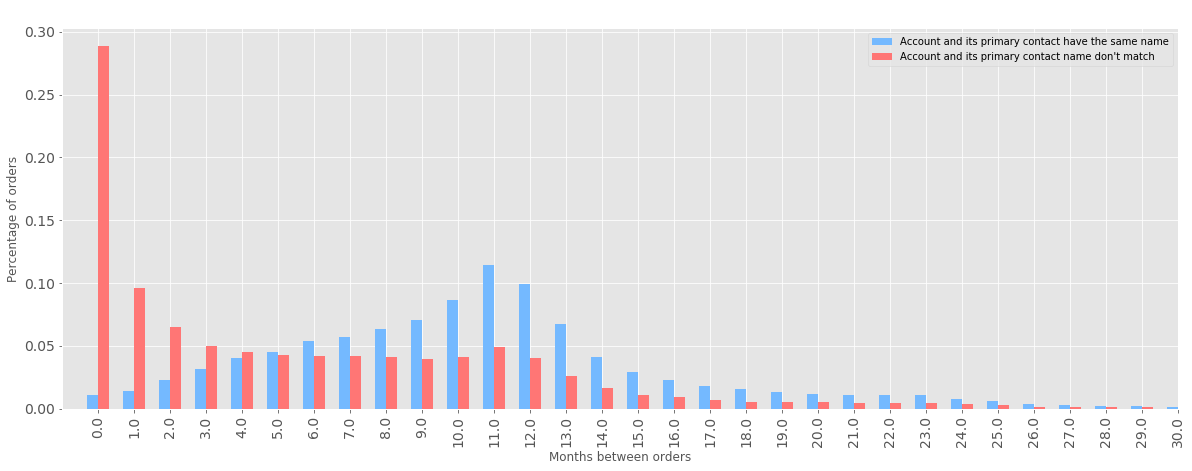
\includegraphics[width=15cm]{images/account-contact-name-orders.png}
    \caption{Number of months between two orders related to the account-contact name}
    \label{fig:account-contact-name-orders}
\end{figure}

Regarding the \texttt{Building} entity, it holds information about the building of a contact (house, offices, cottage, ...). Even if not all contacts have such link (80.84\% of contacts are linked to at least one building), this entity will be used to build new features modeling the amount of product stocked and used, as detailed in section \ref{sec:ml-features}.


\subsection{External data}\label{sec:external-data}
In addition to the data coming from Dynamics 365, there are two important variables to take into account for predicting the date of customer next order: price and weather. This two datasets will be used to created new features, detailed in section \ref{sec:ml-features}.

As explained in section \ref{sec:use-case}, the prices are mainly dependant of the stock market, which can change every day. Therefore, it has been observed by \textit{Company A} that when the price is going down, more orders are being made and when the price is going up, customers would rather wait a bit more, consume their stock and waiting for a decrease to place a new order. A dataset containing the monthly prices of \textit{Company A} between 2013 and 2018 has been created. Unfortunately, it was not possible to compare this data with the monthly prices set by each competitors.

Weather data has also an influence on the ordering patterns of clients, as shown in section \ref{sec:crm-orders}. Weather data has been provided by \texttt{MeteoSwiss} with several daily metrics associated to the 20 meteorological station across Switzerland (weather, precipitations, wind, ...). Based on the primary contact address, each \texttt{account} object has been linked to one of those station and among all metrics, only the weather degrees \big[°C\big] have been used.


\subsection{Shape data for Machine Learning }\label{sec:data-shape-for-ml}


\begin{center}\textbf{--> HERE <---}\end{center}


data from crm
weather
price
one entry per month



% -------------------------------- Section: Customer Jounrey + Feature engineering
\section{Feature engineering} \label{sec:ml-features}

feature engineering
Customer journey




% -------------------------------- Section: Machine Learning Experimentation
\section{Machine Learning Experimentation} \label{sec:ml-experimentation}
\lipsum[1]

\subsection{Linear models}
\lipsum[2]

\subsection{Neural Networks}
\lipsum[3]

\subsection{Best model analysis}
\lipsum[3]


% -------------------------------- Section: Deployment
\section{Deployment} \label{sec:crm-deployment}
How to use machine learning predictions within a Dynamics 365 CRM, based on Azure products

\subsection{Azure Architecture}
\lipsum[2]

\subsection{Integration with Dynamics 365}
\lipsum[3]


% -------------------------------- Section: Further Work
\section{Further Work} \label{sec:use-case-further-work}
\lipsum[1]

% -------------------------------- Section: Conclusion
\section{Conclusion} \label{sec:use-case-conclusion}
\lipsum[1]